\ctitle{Fault Tolerance Basics}

This chapter is based on Ch. 2 in Real-Time Systems and Programming Languages 4E (BW).

\sepline

\paragraph{Reliability}\index{reliability} A measure of the success with which the system conforms to some authoritative specification of its behaviour.

\paragraph{Failure vs Fault vs Error} A few definitions:
\begin{itemize}
  \item \textit{Fault:}\index{failure} A mechanical or algorithmic cause which, given the right conditions, produce an unexpected or incorrect result.
  \item \textit{Error:}\index{fault} An internal unexpected problem in a system, caused by activation of a fault.
  \item \textit{Failure:}\index{error} System deviation from its specification.
\end{itemize}

\tikzstyle{process} = [rectangle, minimum width=1cm, minimum height=1cm, text centered, text width=1cm, draw=black, fill=blue!10]

\tikzstyle{arrow} = [thick,->,>=stealth]

% --- %

\resizebox{8cm}{!} {%
  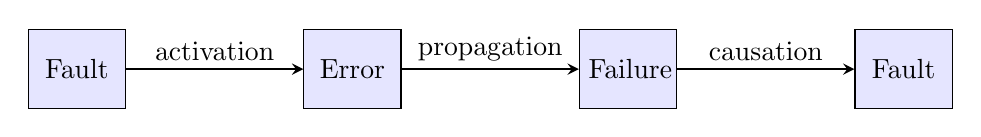
\begin{tikzpicture}[align=center, node distance=1cm]

  \node (f1) [process] {Fault};
  \node (f2) [process, right of=f1, xshift=2.5cm] {Error};
  \node (f3) [process, right of=f2, xshift=2.5cm] {Failure};
  \node (f4) [process, right of=f3, xshift=2.5cm] {Fault};

  % --- %

  \draw [arrow] (f1) -- node[anchor=south, yshift=-0.025cm] {activation} (f2);
  \draw [arrow] (f2) -- node[anchor=south, yshift=-0.025cm] {propagation} (f3);
  \draw [arrow] (f3) -- node[anchor=south, yshift=-0.025cm] {causation} (f4);

  \end{tikzpicture}
}


\paragraph{Types of fault}
\begin{itemize}[nolistsep,noitemsep]
  \item \textit{Transient faults:} Occur at a particular time, remain in the system for a period, then disappear afterwards. An example of this is radioactivity.
  \item \textit{Permanent faults:} A fault that persists in the system until it is fixed. All software faults are permanent faults.
  \item \textit{Intermittent faults:} A special case of transient faults that occur repeatedly. Overheating is an example.
\end{itemize}

\paragraph{Failure modes}\index{failure modes} Two general domains of failure modes can be identified:
\begin{itemize}[nolistsep,noitemsep]
  \item \textit{Value failure:} The output is wrong or even corrupted/unusable.
  \item \textit{Time failure:} The service is delivered at the wrong time.
\end{itemize}

% TODO: insert failure mode classification figure

\paragraph{Fault prevention}\index{fault prevention} Attempts to eliminate any possibility of faults creeping into a system before it goes operational. Two stages: fault avoidance and fault removal.

\paragraph{Fault tolerance}\index{fault tolerance} Enables the system to continue functioning even in the presence of faults. Different levels of faults can be provided by a system:
\begin{itemize}[nolistsep,noitemsep]
  \item \textit{Full fault tolerance:} The system continues to operate in the presence of faults, albeit for a limited period, with no significant loss of functionality or performance.
  \item \textit{Graceful degradation:} The system continues to operate in the presence of errors, accepting a partial degradation of functionality or performance during recovery or repair.
  \item \textit{Fail safe:} The system maintains its integrity while accepting a temporary halt in its operation.
\end{itemize}

\paragraph{Redundancy}\index{redundancy} All techniques for achieving fault tolerance rely on extra elements (redundancy) introduced into the system to detect and recover from faults. Can be implemented in both software and hardware.

Distinguish between static and dynamic redundancy for hardware:
\begin{itemize}[nolistsep,noitemsep]
  \item \textit{Static:}\index{redundancy!static} Redundant components are used inside a system (or subsystem) to hide the effects of faults. (error masking)
  \item \textit{Dynamic:}\index{redundancy!dynamic} The redundancy supplied inside a component which indicates explicitly or implicitly that the output is in error. (error detection)
\end{itemize}


\paragraph{N-version programming}\index{N-version programming} Defined as the independent generation of $N$ (where $N \geq 2$) functionally equivalent programs from the same initial specification. The programs execute concurrently without interaction, and the results (compared by a driver process) should be identical. However, if they do not produce the same result the driver might choose the most common result, ask the processes to compute it again, or simply terminate the faulty process.

To achieve diversity, different programming languages and different development environments could be used. Alternatively, if the same language is used, different compilers and support environments should be employed. ($N$-version programming is the software equivalent of static redundancy.)

Downsides to this solution:
\begin{itemize}[nolistsep,noitemsep]
  \item In a real-time system, the driver process and different programs may need to communicate -- introducing a communication module.
  \item High cost of introducing a redundant language/hardware etc.
  \item Most software faults originate from the specification -- all $N$ versions may suffer from the same fault.
\end{itemize}

\paragraph{Dynamic redundancy}\index{redundancy!dynamic} The redundant components only come into action when an error has been detected. Has four stages presented in the following four paragraphs.

\paragraph{Error detection} Two classes of error detection techniques can be identified. You should know this list by heart!
\begin{itemize}[nolistsep,noitemsep]
  \item Environmental detection
  \item Application detection. Since the recovery system is not continually running, there needs to be some way to detect a fault. There are many triggers that could be used.
  \begin{itemize}[nolistsep,noitemsep]
    \item Replication checks --
    \item Timing checks --
    \item Reversal checks --
    \item Coding checks --
    \item Reasonableness checks --
    \item Structural checks --
    \item Dynamic reasonableness checks --
  \end{itemize}
\end{itemize}

\paragraph{Damage confinement and assessment} Concerned with structuring the system as to minimize the damage caused by a faulty component (also known as firewalling). Two techniques: modular decomposition and atomic actions.

\paragraph{Error recovery}\index{error recovery} Once an error situation has been detected and the damage assessed, error recovery procedures must be initiated.

\textit{Forward error recovery:}\index{error recovery!forward} Attempts to continue from an erroneous state by making selective corrections to the system state. Although it is efficient, it is system specific and depends on accurate predictions of the location and cause of errors.

\textit{Backward error recovery:}\index{error recovery!backward} Relies on restoring the system to a safe state (recovery point) previous to that in which the error occurred. Straightforward if no threads, but gets complicated with more threads. A big advantage: Does not rely on finding the location or cause of fault. A huge disadvantage: It is difficult to undo eg. a missile launch...

\paragraph{Fault treatment} Two stages: Fault location and system repair.

\paragraph{Domino effect}\index{domino effect} If one thread needs to roll back due to an error, then it must undo the communication with the other threads. This may propagate further back and forth, and will end up in multiple threads having to roll back as well.

\paragraph{Recovery blocks}\index{recovery blocks} Blocks in the normal programming sense except that at the entrance is an automatic \textit{recovery point} and at the end an \textit{acceptance test}. (dynamic recovery)

% TODO: insert recovery block figure

\paragraph{Acceptance test}\index{acceptance test} Used to test that the system is in an acceptable state after the execution of the block. It can utilize several of the methods discussed for error detection. If it fails, the program will be restored to the recovery point at the beginning of the block and an alternative module will be executed.

% TODO: a comparison between N-version programming and recovery blocks, failfast, failure mode merging
